\documentclass{article}
\usepackage{amsmath}
\usepackage{mathtools}
\usepackage{gensymb}
\usepackage[a4paper,inner=1.5cm,outer=1.5cm,top=2cm,bottom=0.5cm]{geometry} 
\usepackage{xcolor}                    
\usepackage{tikz}                           
\usepackage{multicol}
\usepackage{pgfplots}
\usetikzlibrary{calc}
\usetikzlibrary{intersections}
\usetikzlibrary{intersections,calc,angles,quotes}
\usetikzlibrary{shapes,arrows,positioning,decorations.pathreplacing,calc}
\usetikzlibrary{calc,angles,positioning,intersections,quotes,decorations.markings}
\usepackage{tkz-euclide}
\usetikzlibrary{backgrounds}
\usetikzlibrary{calc,through}
\usetikzlibrary{angles}
\usetikzlibrary{fadings}
\usetikzlibrary{shapes.geometric}
\usetikzlibrary{shapes.symbols}
\usepackage{draftwatermark}
\usepackage{mathptmx}

\SetWatermarkText{\textcolor{black!30}{Mathema Shukur}}
\SetWatermarkFontSize{2 cm}
\usepackage[utf8]{inputenc}
\usepackage{fontspec}

\setmainfont{[Kalpurush.ttf]}
\newfontface{\en}{[Arial.ttf]} %%this is optional, if you want to use a secondary font. Any english font is supported
\newlength\Radius
\setlength\Radius{4cm}
\begin{document} 
	\Large
	\textcolor{red}{Welcome To} 
	\\
	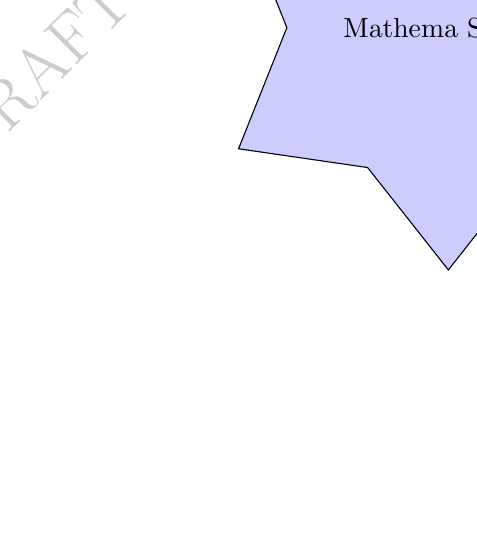
\begin{tikzpicture}
		\tikz \node [fill=blue!20,star,star points=6,draw] {Mathema Shukur };
	\end{tikzpicture}
	\\
	যাদের জন্যে প্রযোজ্যঃ  	\textcolor{magenta}{একাদশ ও দ্বাদশ শ্রেণীর শিক্ষার্থী} \\
	বিষয়ঃ \textcolor{magenta}{উচ্চতর গণিত ১ম পত্র} \\
	অধ্যায়ঃ \textcolor{magenta}{৩-সরলরেখা}\\ 
	Subtopicঃ  \textcolor{magenta}{সরলরেখার ঢাল নির্ণয় করা slope of a line  }\\
	\\
	ঢাল= ( y এর মানের পরিবর্তন )/ ( x এর মানের পরিবর্তন )\\
	\\
	$m=\frac{\mbox{rise}}{\mbox{run}}=\frac{y_1-y_2}{x_1-x_2}$\\ 
\\
\begin{tikzpicture}[transform shape,scale=1]
	\draw [-latex,thick](-3,0) -- (8,0) node[right] {$x$} coordinate(x axis);
	\draw [-latex,thick](0,-3) -- (0,8) node[above] {$y$} coordinate(y axis);
	\fill[black] (0,0) circle (0.5 mm);
	\node at (0.3,-0.3) {$\textcolor{purple}{O}$};	
	\node at (2.5,2) {$\textcolor{blue}{\mbox{run}}$};	
	\node at (4,4) {$\textcolor{green}{\mbox{rise}}$};		
		\node at (0.5,2.5) {$\textcolor{red}{A(x_1,y_1)}$};		
			\node at (4.5,5.5) {$\textcolor{red}{B(x_2,y_2)}$};	
	\draw[very thick,red] (4.5,7.5)--(-1.5,-2.5);
	\draw[very thick,blue] (1.5,2.5)--(3.5,2.5);
		\draw[very thick,green] (3.5,2.5)--(3.5,5.8);
\end{tikzpicture}
\begin{multicols}{2}
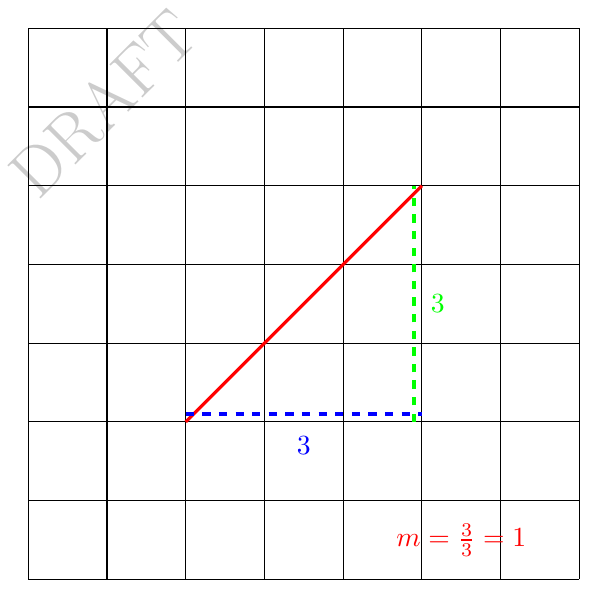
\begin{tikzpicture}[transform shape,scale=1]
	\draw (0,0) grid (7,7);
	\draw[very thick,red] (2,2)--(5,5);
	\draw[very thick,blue,dashed] (2,2.1)--(5,2.1);
	\draw[ very thick,green,dashed] (4.9,2)--(4.9,5);
	\node at (3.5,1.7) {$\textcolor{blue}{3}$};
	\node at (5.2,3.5) {$\textcolor{green}{3}$};
	\node at (5.5,0.5) {$\textcolor{red}{m=\frac{3}{3}=1}$};
\end{tikzpicture}
\\
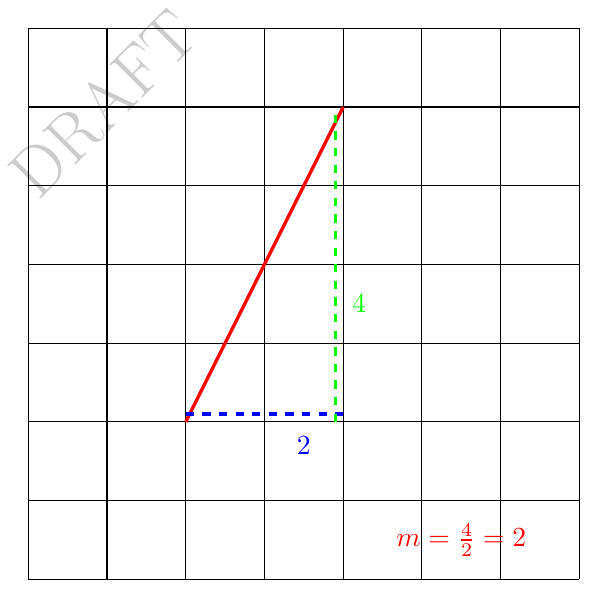
\begin{tikzpicture}[transform shape,scale=1]
	\draw (0,0) grid (7,7);
	\draw[very thick,red] (2,2)--(4,6);
	\draw[very thick,blue,dashed] (2,2.1)--(4,2.1);
	\draw[ very thick,green,dashed] (3.9,2)--(3.9,6);
	\node at (3.5,1.7) {$\textcolor{blue}{2}$};
	\node at (4.2,3.5) {$\textcolor{green}{4}$};
	\node at (5.5,0.5) {$\textcolor{red}{m=\frac{4}{2}=2}$};	
\end{tikzpicture}
\end{multicols}
\begin{multicols}{2}
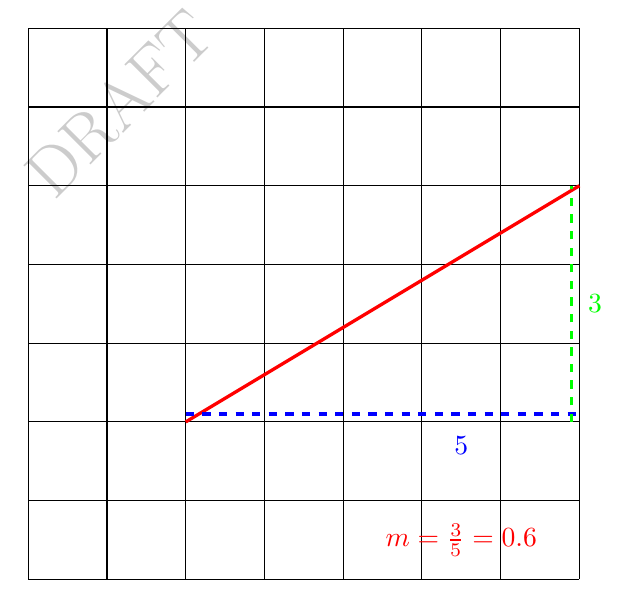
\begin{tikzpicture}[transform shape,scale=1]
	\draw (0,0) grid (7,7);
	\draw[very thick,red] (2,2)--(7,5);
	\draw[very thick,blue,dashed] (2,2.1)--(7,2.1);
	\draw[ very thick,green,dashed] (6.9,2)--(6.9,5);
	\node at (5.5,1.7) {$\textcolor{blue}{5}$};
	\node at (7.2,3.5) {$\textcolor{green}{3}$};
	\node at (5.5,0.5) {$\textcolor{red}{m=\frac{3}{5}=0.6}$};
\end{tikzpicture}
\\
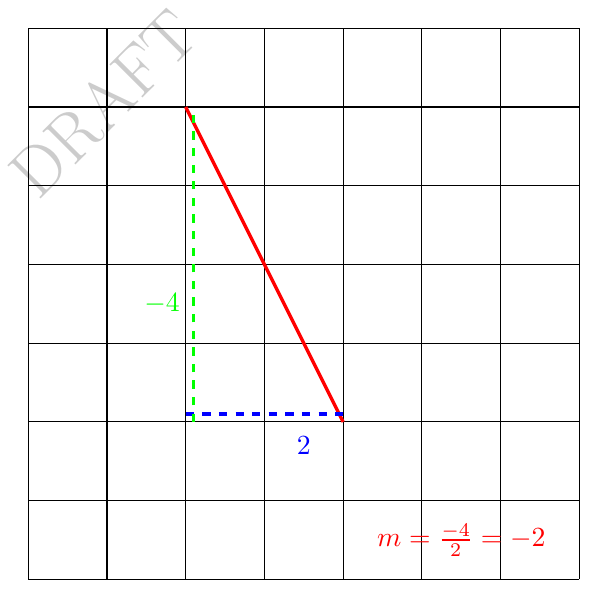
\begin{tikzpicture}[transform shape,scale=1]
	\draw (0,0) grid (7,7);
	\draw[very thick,red] (4,2)--(2,6);
	\draw[very thick,blue,dashed] (2,2.1)--(4,2.1);
	\draw[ very thick,green,dashed] (2.1,2)--(2.1,6);
	\node at (3.5,1.7) {$\textcolor{blue}{2}$};
	\node at (1.7,3.5) {$\textcolor{green}{-4}$};
	\node at (5.5,0.5) {$\textcolor{red}{m=\frac{-4}{2}=-2}$};
\end{tikzpicture}
\end{multicols}
\begin{multicols}{2}
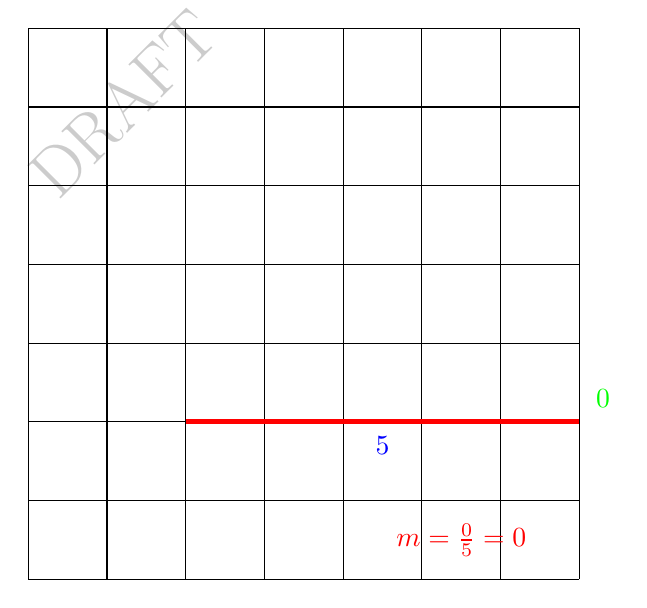
\begin{tikzpicture}[transform shape,scale=1]
	\draw (0,0) grid (7,7);
	\draw[very thick,red] (2,2.01)--(7,2.01);
	\draw[very thick,red] (2,2)--(7,2);
	\node at (4.5,1.7) {$\textcolor{blue}{5}$};
	\node at (7.3,2.3) {$\textcolor{green}{0}$};
	\node at (5.5,0.5) {$\textcolor{red}{m=\frac{0}{5}=0}$};
\end{tikzpicture}
\\
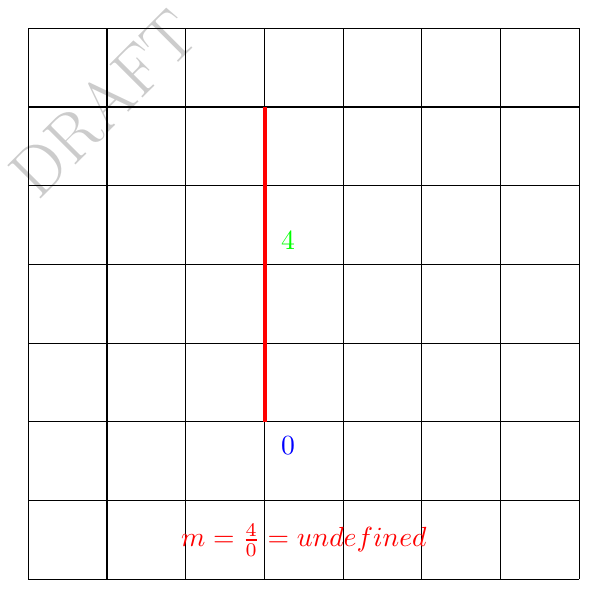
\begin{tikzpicture}[transform shape,scale=1]
	\draw (0,0) grid (7,7);
	\draw[very thick,red] (3,2)--(3,6);
	\draw[very thick,red] (3.01,2)--(3.01,6);
	\node at (3.3,1.7) {$\textcolor{blue}{0}$};
	\node at (3.3,4.3) {$\textcolor{green}{4}$};
	\node at (3.5,0.5) {$\textcolor{red}{m=\frac{4}{0}=undefined}$};
\end{tikzpicture}
\end{multicols}
\textcolor{blue}{$(x_1,y_1)$ ও $(x_2,y_2)$ বিন্দুগামী সরলরেখার ঢাল  $m=\frac{y_1-y_2}{x_1-x_2}$}\\
\\ 
বরিশাল বোর্ড-২০২১\\
একটি সরলরেখা $(5,5)$ ও $(3,7)$ বিন্দুগামী হলে রেখাটির ঢাল কত? \\
\\
$(x_1,y_1)=(5,5)$,\qquad $(x_2,y_2)=(3,7)$\\
\\
ঢাল= $m=\frac{y_1-y_2}{x_1-x_2}=\frac{5-7}{5-3}=\frac{-2}{2}=-1$\\
\\ 
\textcolor{blue}{$ax+by+c=0$  সরলরেখার ঢাল  $m=-\frac{a}{b}$}\\
\\
ঢাকা বোর্ড-২০২১\\ 
$2x-3y+6=0$ সরলরেখাটির ঢাল কত? \\
$a=2$,\qquad  $b=-3$\\
\\
ঢাল $m=-\frac{a}{b}=-\frac{2}{-3}=\frac{2}{3}$\\ 
\\ 
কোনো সরলরেখা x অক্ষের ধনাত্মক দিকের সাথে যে কোণ উৎপন্ন করে , তার ত্রিকোণমিতিক ট্যাঞ্জেন্টের মানকে সরলরেখাটির ঢাল বলে । \\
\\
\textcolor{blue}{$m= \tan \theta$}\\ 
\\ 
ইসলামী  বিশ্ববিদ্যালয় ভর্তি পরীক্ষা -২০১৬-২০১৭\\ 
$(3,-1)$ ও $(4,-2)$ বিন্দুদ্বয়ের সংযোগ রেখা  $x-$ অক্ষের সাথে কত কোণ উৎপন্ন করে। \\
\\
$(x_1,y_1)=(3,-1)$,\qquad $(x_2,y_2)=(4,-2)$\\
\\
ঢাল= $m=\frac{y_1-y_2}{x_1-x_2}=\frac{-1+2}{3-4}=\frac{1}{-1}=-1$\\
\\
\begin{align*}
	m&=\tan \theta \\
	\\
	-1&=\tan \theta\\
	\\
	\tan \theta& = -\tan 45\degree \\
	\\
	\tan \theta &=\tan (180\degree-45\degree)\\
	\\
	\theta& =135\degree\\
\end{align*}
\\
	\begin{tikzpicture}[transform shape,scale=1]
	\draw [-latex,thick](-6,0) -- (6,0) node[right] {$x$} coordinate(x axis);
	\draw [-latex,thick](0,-6) -- (0,6) node[above] {$y$} coordinate(y axis);
	\fill[black] (0,0) circle (0.5 mm);
	\node at (0.3,-0.3) {$\textcolor{purple}{O}$};	
	\draw[very thick,magenta] (3,-1)--(4,-2);
		\draw[very thick,magenta,dashed] (3,-1)--(-3,5);
	\node at (3.5,0.4) {$\textcolor{blue}{135\degree}$};	
	\node at (4,-1) {$\textcolor{magenta}{(3,-1) }$};	
	\node at (4.5,-2.5) {$\textcolor{magenta}{(4,-2) }$};
	\node at (5,5.5) {$\textcolor{magenta}{A}$};
	\draw[color=blue,ultra thick, ->] (3,0) arc (0:135:1cm);
\end{tikzpicture}
\\
বরিশাল বোর্ড-২০২১\\ 
$2x+2y-\sqrt{5}=0$ সরলরেখাটি  $x-$ অক্ষের ধনাত্মক দিকের সাথে কত ডিগ্রী কোণ উৎপন্ন করে ? \\
\\ 
\textcolor{blue}{$ax+by+c=0$  সরলরেখার ঢাল  $m=-\frac{a}{b}$}\\
\\ 
$a=2$,\qquad $b=2$\\
\\
$m=-\frac{a}{b}=-\frac{2}{2}=-1$\\
\\ 
\begin{align*}
	m&=\tan \theta \\
	\\
	-1&=\tan \theta\\
	\\
	\tan \theta& = -\tan 45\degree \\
	\\
	\tan \theta &=\tan (180\degree-45\degree)\\
	\\
	\theta& =135\degree\\
\end{align*}
\\
	\begin{tikzpicture}[transform shape,scale=1]
	\draw [-latex,thick](-6,0) -- (6,0) node[right] {$x$} coordinate(x axis);
	\draw [-latex,thick](0,-6) -- (0,6) node[above] {$y$} coordinate(y axis);
	\fill[black] (0,0) circle (0.5 mm);
	\node at (0.3,-0.3) {$\textcolor{purple}{O}$};	
	\draw[very thick,magenta] (-4,5)--(5,-4);
	\node at (2.5,0.4) {$\textcolor{blue}{135\degree}$};	
	\node at (4.2,-1) {$\textcolor{magenta}{2x+2y-\sqrt{5}=0 }$};	
	\node at (5,5.5) {$\textcolor{magenta}{A}$};	
	\draw[color=blue,ultra thick, ->] (2,0) arc (0:135:1cm);
\end{tikzpicture}
\\
বরিশাল বোর্ড-২০১৯\\
\\ 
$x-\sqrt{3}y-\sqrt{3}=0$ সরল রেখাটির ঢাল কত? \\
\\ 
$m=-\frac{1}{-\sqrt{3}}=\frac{1}{\sqrt{3}}=\tan 30\degree$\\
\\ 
	\begin{tikzpicture}[transform shape,scale=1]
	\draw [-latex,thick](-4,0) -- (8,0) node[right] {$x$} coordinate(x axis);
	\draw [-latex,thick](0,-4) -- (0,4) node[above] {$y$} coordinate(y axis);
	\fill[black] (0,0) circle (0.5 mm);
	\node at (0.3,-0.3) {$\textcolor{purple}{O}$};	
	\draw[very thick,magenta] (-3.5,-3)--(6,2.25);
	\node at (3.5,0.4) {$\textcolor{blue}{30\degree}$};		
	\node at (2.3,-1) {$\textcolor{magenta}{x-\sqrt{3}y-\sqrt{3}=0}$};			
	\draw[color=blue,ultra thick, ->] (3,0) arc (0:30:1cm);
\end{tikzpicture}
\\
ইসলামী  বিশ্ববিদ্যালয় ভর্তি পরীক্ষা -২০১৭-২০১৮\\ 
(1) একটি সরলরেখা $x-$ অক্ষের ঋণাত্মক অংশে $120\degree $ কোণ উৎপন্ন করলে ঐ সরলরেখার ঢাল কত? \\
\\ 
\textcolor{blue}{$m=\sqrt{3}$}\\
\\ 
(2) রাজশাহী বোর্ড-২০১৯\\
$x-\sqrt{3}y=7$ সরলরেখার ঢাল কত?\\
\\ 
\textcolor{blue}{$m=\frac{1}{\sqrt{3}}$}\\
\\ 
(3) চট্রগ্রাম বোর্ড-২০১৯\\
$x+y+3=0$ সরলরেখাটি x-  অক্ষের ধনাত্মক দিকের সাথে কত ডিগ্রী কোণ উৎপন্ন করে । \\
\\
\textcolor{blue}{$\theta=135\degree$}\\
\\
(4) বরিশাল বোর্ড-২০১৯\\
$y+x=0$ সরলরেখাটি x-  অক্ষের ধনাত্মক দিকের সাথে কত ডিগ্রী কোণ উৎপন্ন করে । \\
\\
\textcolor{blue}{$\theta=135\degree$}\\
\\
(5) ঢাকা বোর্ড-২০১৯\\
$A(-4,0)$ ও $B(0,-3)$ বিন্দুর সংযোজক রেখার ঢাল নির্ণয় কর।\\
\\ 
\textcolor{blue}{$m=\frac{3}{4}$}\\
\\ 
(6) যশোর বোর্ড-২০১৭\\
$3x+4y+1=0$ সরলরেখার ঢাল কত?\\  
\\ 
\textcolor{blue}{$m=-\frac{3}{4}$}\\
\\ 
(7) সিলেট বোর্ড-২০১৭\\
$4x-3y+5=0$ সরলরেখার ঢাল কত?\\
\\
(8) দিনাজপুর  বোর্ড-২০১৭\\
$4x-2y=6$ সরলরেখার ঢাল কত?\\
\\
(9) রাজশাহী  বোর্ড-২০১৭\\
$3x-5y+1=0$ সরলরেখার ঢাল কত?\\
\\
(10)  দিনাজপুর বোর্ড-২০১৯\\
$2x+4y-1=0$ রেখার ঢাল নির্ণয় কর।\\
\\
(11)  চট্রগ্রাম বোর্ড-২০১৯\\ 
$x+y+3=0$ সরল রেখাটি x- অক্ষের ধনাত্মক দিকের সাথে কত ডিগ্রী কোণ উৎপন্ন করে।  \\
\end{document}